\section{DM vs. ULDM}

\begin{frame}{Dark Matter (DM)}

\begin{center}
        \textcolor{yellow}{\fbox{What about dark matter?}} 
\end{center}


\begin{itemize}
    \item \textcolor{blue2}{ \small Cosmic density:  DM $\rightarrow{26 \%}$; ordinary matter $\rightarrow{6 \%}$; vacuum energy $\rightarrow{68 \%}$  }
    
    \item \textcolor{green2}{\small Local density: of DM $\rightarrow{}$ one proton * cm$^{-3}$ / one solar mass * lightyear$^{-3}$ }
    \item \textcolor{red2}{\small Local velocity dispersion of DM around $\sigma_v = 200 km/s$}
    \item \textcolor{violet2}{\small DM nonrelativistic $v \sim c$ and negligible pressure. For boson $\lambda_{Br}$ small comparaed to galaxy clustering scale }
    \item \textcolor{orange2}{\small DM long before CBM formed, before was 1 year old. For light bosonic DM (axion) $\rightarrow{}$ lastest epoch of particle creation}
    \item \textcolor{yellow}{\small DM cannot interact with itself or with ordinary matter strongly}
\end{itemize}
    
\end{frame}
\begin{frame}{Frame Title}
    
    \begin{block}{Abstract}
    \centering
        There's a block
    \end{block}

        \centering
        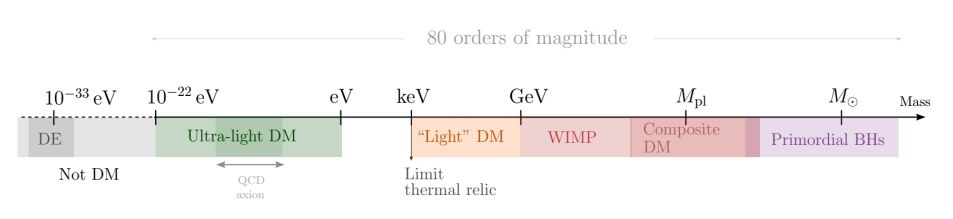
\includegraphics[width = 1\textwidth]{images/DM_particles.jpg}\\
        \footnotesize \textcolor{yellow}{Figure 1:} Sketch (not to scale) of possibly DM models
    \end{frame}
    

\begin{frame}{Imagem}
    \centering
        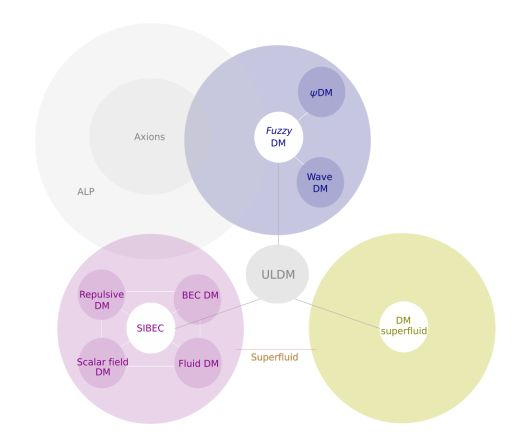
\includegraphics[width = 0.6
        \textwidth]{images/classes_ULDM.jpg}\\
        \footnotesize \textcolor{yellow}{Figure 1:} Sketch (not to scale) of possibly DM models
\end{frame}

\begin{frame}{Frame Title}

        \centering
        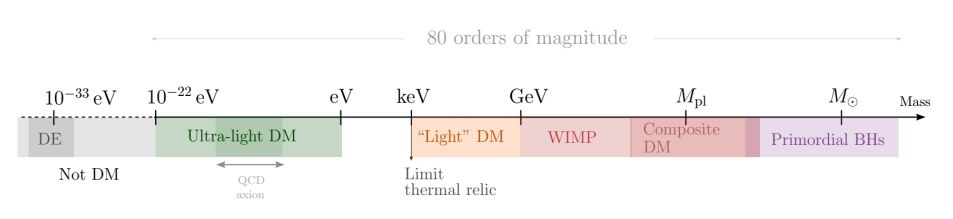
\includegraphics[width = 1\textwidth]{images/DM_particles.jpg}\\
        \footnotesize \textcolor{yellow}{Figure 1:} Sketch (not to scale) of possibly DM models
    \end{frame}
    
 \frame{\sectionpage}



\begin{frame}{Blocks}
\begin{block}{begin block}
There's a block
\end{block}

\begin{alertblock}{begin alertblock}
    there's a alert block 
\end{alertblock}

\begin{exampleblock}{begin example block}
here comes example
\end{exampleblock} 

\end{frame}


\begin{frame}{Blocks}
    
\begin{theorem}
    Here comes a theorem
\end{theorem}

\begin{proof}
    Here comes the proof
\end{proof}


    
\end{frame}